% !TeX TXS-program:compile = txs:///pdflatex/[--shell-escape]

\documentclass[11pt, letterpaper]{article}

\usepackage{minted}
\usepackage[utf8]{inputenc}
\usepackage[T1]{fontenc}
\usepackage{lmodern}
\usepackage{graphicx}
\usepackage{longtable}
\usepackage{wrapfig}
\usepackage{rotating}
\usepackage{amsmath}
\usepackage{textcomp}
\usepackage{amssymb}
\usepackage{hyperref}
\usepackage[round]{natbib}
\usepackage{subcaption}


\title{\bfseries Tarea}
\author{Ángel García Báez}
\date{\today}
\setcounter{tocdepth}{3} 

\begin{document}
	
	% Página de presentación
	\begin{titlepage}
		\centering
		
\includegraphics[width=0.2\textwidth]{logo.png}\par
		\vspace{1cm}
		{\LARGE \bfseries Universidad Veracruzana \par}
		\vspace{1cm}
		{\Large Maestría en Inteligencia Artificial\par}
		\vspace{3cm}
		{\LARGE \bfseries Visión por Computadora \par}
		\vspace{1cm}
		{\Large \bfseries Tarea 12. Clasificación binaria de imagenes de gusanos mediante una red neuronal convolucional en MATLAB \par}
		\vfill
		{\Large \textit{Ángel García Báez}\par}
		\vspace{1cm}
		{\Large Profesor: Dr. Héctor Acosta Mesa \par}
		\vfill
		{\Large \today \par}
	\end{titlepage}
	
	% Página exclusiva para la tabla de contenidos
	\newpage
	\tableofcontents
	\newpage
	
% Sección para el problema 1
\section{Objetivo de la práctica}

Para la presente practica, se cuenta con un conjunto de 93 imágenes en formato .tif de gusanos, de los cuales 48 están etiquetados como "vivos" y 45 están identificados como muertos. A continuación se muestra una muestra de como son estas imágenes.


\begin{figure}[h!]
	\centering
	\begin{minipage}{0.8\textwidth}
		\centering
		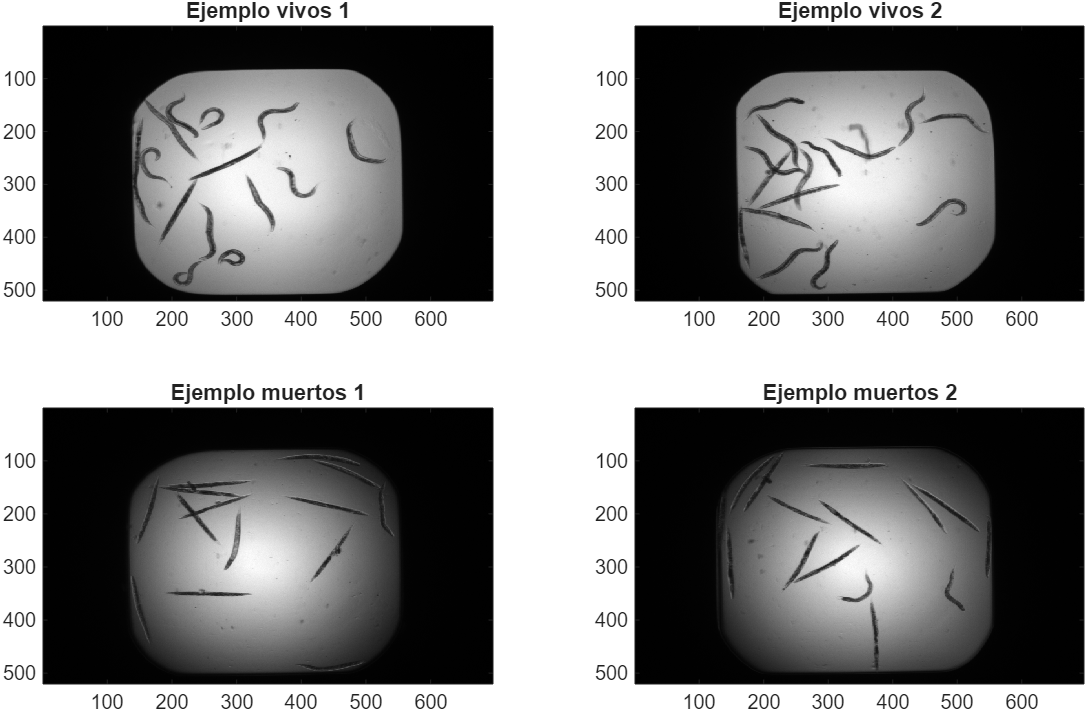
\includegraphics[width=\textwidth]{IMG/R1.png}
		\caption*{Muestra de gusanos vivos y muertos.}
	\end{minipage}\hfill
\end{figure}

Se observan claras diferencias entre el comportamiento de ambas imagenes, para el caso de los gusanos vivos, se percibe movimientos y formas curvas. Para el caso de los gusanos muertos, se perciben en posiciones rectas. \\

Una vez entendido esto, lo que se pide hacer es lo siguiente:


\begin{itemize}
	\item Se pide implementar una metodología usando redes neuronales convolucionales para llevar a cabo la clasificación binaria (vivos o muertos) de las imágenes.
	
	\item Se espera lograr un mínimo de buena clasificación del 90\%
	
\end{itemize}




	
\newpage
	
\section{Metodología}

\subsection{Dividir la base de datos}

En primera instancia, se toma el conjunto de las 93 imágenes y se divide en 2 partes siguiendo la proporción 80-20. El 80\% de los datos (77 imágenes) que se seleccionaron de forma al azar, fueron utilizadas para entrenar al modelo de red neuronal mientras que el restante 20\% (19 imágenes) fueron utilizadas como prueba. Cabe mencionar que se fijo la semilla 64 para replicabilidad.

\subsection{Propuesta para construir la red neuronal}

Para llevar a cabo la clasificación automática de imágenes de gusanos vivos y muertos se pusieron en practica los conceptos expuestos en \cite{wu2017introduction} como introducción a las redes convolucionales en matlab. Se desarrolló una red neuronal convolucional (CNN) en MATLAB como sigue:

\begin{itemize}
	\item Como pre-procesamiento se tomaron todas las imágenes de gusanos vivos y muertos, se estandarizaron en un formato de 100x100 píxeles en escala de grises con ayuda de la función augmentedImageDatastore() de MATLAB.

	\item La arquitectura de la red comienza pidiendo una capa de entrada que recibe las imágenes en escala de grises de tamaño 100x100.
	
	\item Se agregan dos bloques convolucionales, cada uno compuesto por una capa de convolución 2D que detecta patrones espaciales locales mediante filtros 2D.
	
	\item Se aplica una capa de normalización por lotes que estabiliza el aprendizaje y acelera la convergencia.
	
	\item Se agrega una capa con la función de activación ReLU que introduce no linealidad al modelo.
	
	\item Cada bloque se completa con una capa de submuestreo con maxPooling2dLayer que va reduciendo la dimensionalidad espacial y conservando las características más importantes.
	
	\item Se incluye una capa completamente conectada al final de la extracción de caracteristicas con 2 neuronas de salida, correspondientes a las clases de los gusanos.
	
	\item Se usa una capa softmax para convertir las salidas en probabilidades que finalmente terminan en una capa de clasificación que permiten a la red decir si una imagen presenta gusanos vivos o no.
	
	
\end{itemize}

  El entrenamiento de la red se realizó con el algoritmo de optimización Adam, configurando un máximo de 20 épocas y una frecuencia de validación cada 5 iteraciones para monitorear el rendimiento. Se habilitó la visualización del progreso del entrenamiento mediante gráficos, lo que permitió observar la evolución de la precisión y la pérdida. Esta configuración balancea simplicidad y eficiencia, siendo adecuada para un problema binario de clasificación con imágenes de tamaño reducido y características visuales distinguibles.


\newpage
	
\section{Resultados}

\subsection{Proceso de entrenamiento de la red}

A continuación se muestra el comportamiento de la red durante su entrenamiento hasta lograr una convergencia estable:


\begin{figure}[h!]
	\centering
	\begin{minipage}{1\textwidth}
		\centering
		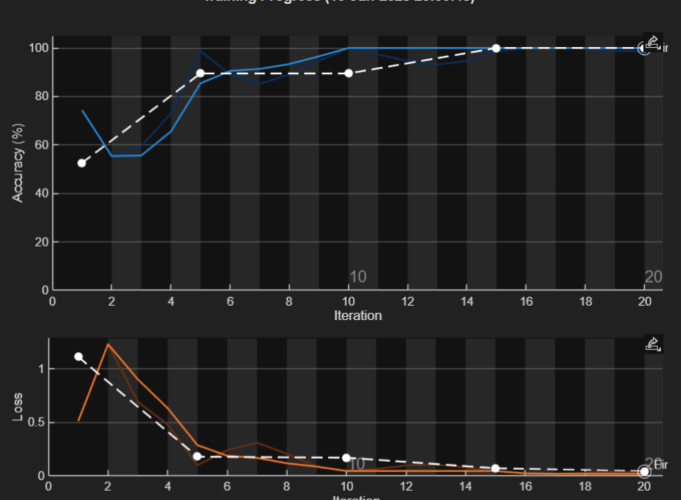
\includegraphics[width=1\textwidth]{IMG/G1.png}
	\end{minipage}
	\caption{Proceso de entrenamiento.}
	\label{fig:f2}
\end{figure}

El gráfico muestra el desempeño de la red neuronal con el conjunto de prueba a lo así como la función de perdida a lo largo de 20 iteraciones.

\newpage

\subsection{Matriz de confusión}

A continuación se muestra la matriz de confusión que reporta la red neuronal al clasificar el conjunto de prueba.

\begin{figure}[h!]
	\centering % Esto centrará la imagen en la página.
	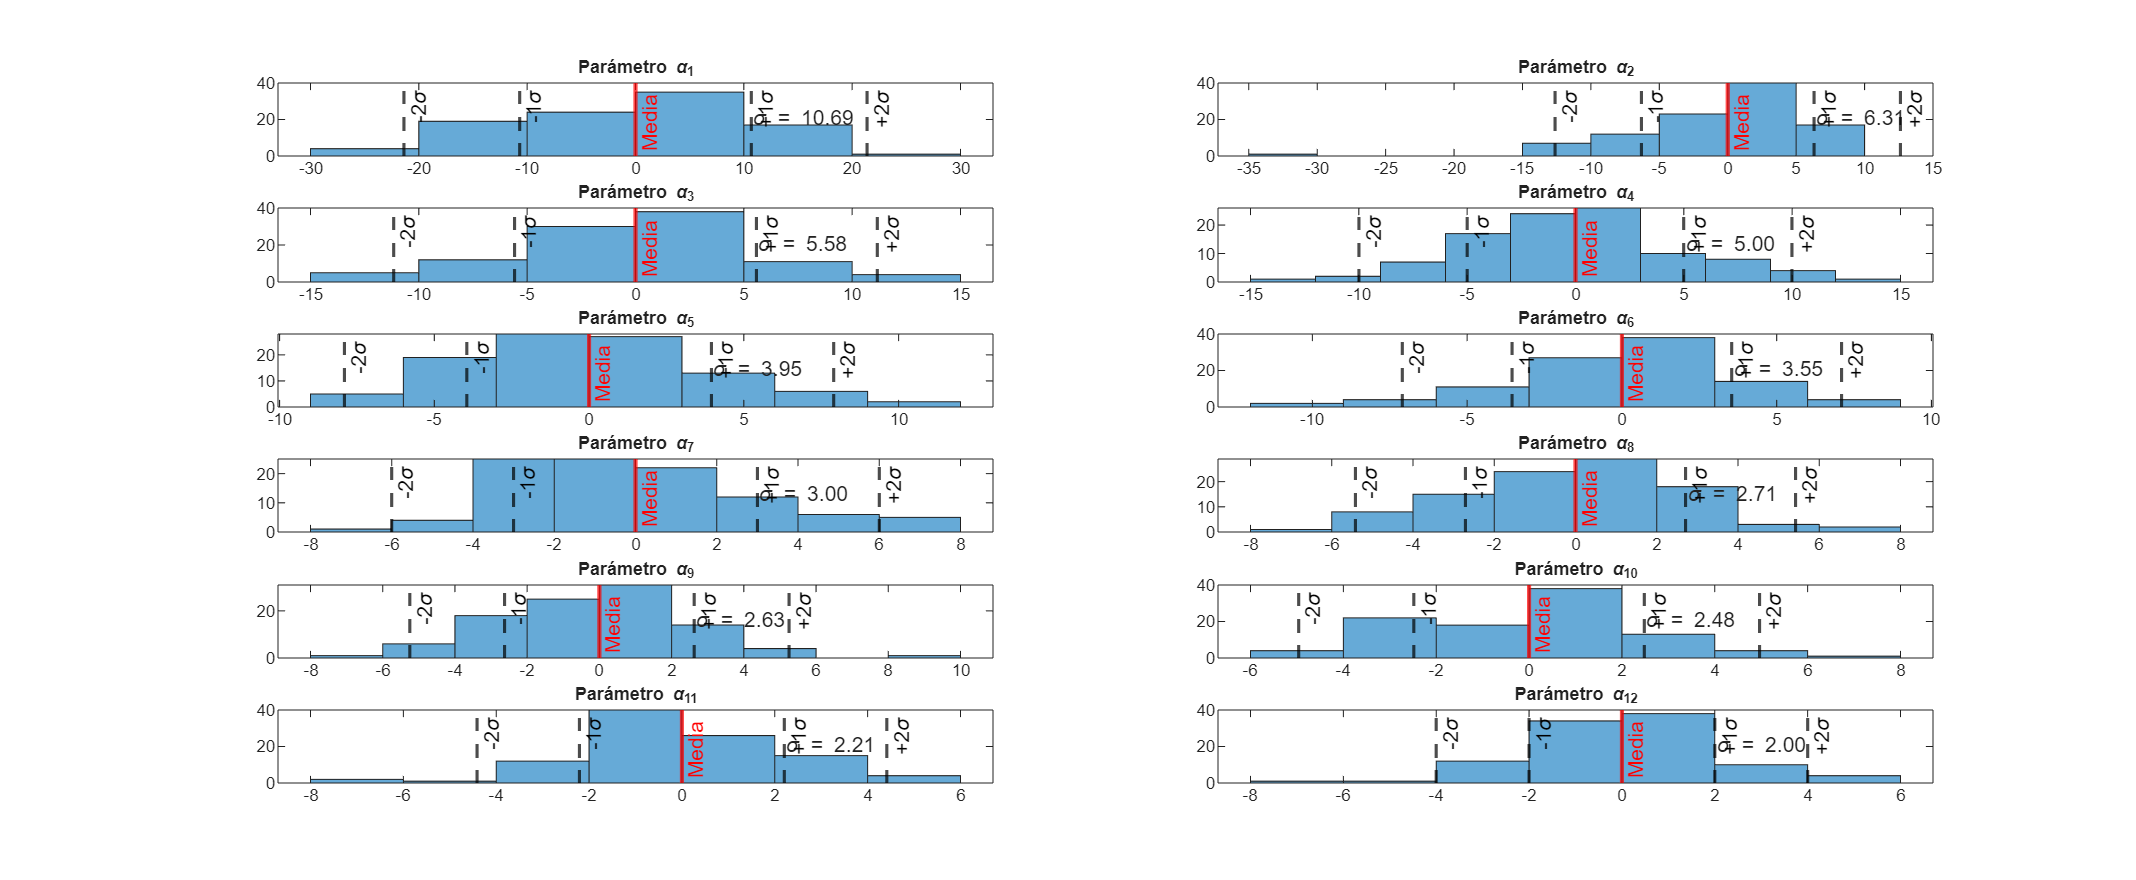
\includegraphics[width=1.35\textwidth]{IMG/G2.png} % Ajusta el ancho aquí, por ejemplo a 90% del ancho del texto.
	\caption{Matriz de confusión.}
	\label{fig:f3}
\end{figure}

Se observa que la red tiene un desempeño perfecto para predecir correctamente al conjunto de prueba, logrando una precisión del 100\%.



\newpage
	
\section{Conclusiones}

Después de haber realizado la implementación del problema y obtener los resultados esperados (una clasificación mayor al 90\%) cabe reflexionar lo importante que es la calibración de la red neuronal, puesto que su funcionamiento es enteramente de caja negra. Se puede llegar a un resultado satisfactorio y saber que operaciones se estan aplicando, pero la calibración de los pesos de dicha red y la forma en que extraer caracteristicas a un nivel tan abstracto, resulta un total misterio que pese a ser bueno en su trabajo, resulta poco explicable.	

\newpage

	
\section{Referencias}  % Sección numerada de referencias
\bibliographystyle{apalike}  % Estilo de citas (puedes cambiarlo)
\bibliography{Biblio}        % Nombre del archivo BibTeX (sin extensión)

\newpage
	
\section{Anexos}	

\subsection{Implementación  en MATLAB de la red convolucional}


\begin{minted}[linenos,firstnumber=1]{matlab}
%% Mostrar una muestra de imagenes %%
rutae = "WormData.csv";
labelsTable = readtable(rutae);
% Filtrar las imágenes 'alive'
aliveFiles = labelsTable(strcmp(labelsTable.Status, 'alive'), :);
% Filtrar las imágenes 'dead'
deadFiles = labelsTable(strcmp(labelsTable.Status, 'dead'), :);
%% Seleccionar las primeras 2 de cada tipo %%
base = "WormImages\";
subplot(2,2,1)
imagesc(imread(strcat(base,aliveFiles.File{1})))
title("Ejemplo vivos 1")
subplot(2,2,2)
imagesc(imread(strcat(base,aliveFiles.File{2})))
title("Ejemplo vivos 2")
subplot(2,2,3)
imagesc(imread(strcat(base,deadFiles.File{1})))
title("Ejemplo muertos 1")
subplot(2,2,4)
imagesc(imread(strcat(base,deadFiles.File{2})))
title("Ejemplo muertos 2")
colormap("gray")
%% Cargar las imagenes %%
ruta = "WormImages\wormA01.tif"
img = imread(ruta);
%imshow(img)
imagesc(img)
colormap("gray")
% Etiquetas %
rutae = "WormData.csv";
labelsTable = readtable(rutae);
labelsTable;
%% Cargar todas las imagenes %%
imageFolder = "WormImages";
% Crear un arreglo de imagenDatastore
imds = imageDatastore(fullfile(imageFolder), ...
'IncludeSubfolders', false, ...
'FileExtensions', '.tif', ...
'LabelSource', 'none');
% Agregar las etiquetas al datastore
imds.Labels = categorical(labelsTable.Status);
%% Dividir los datos %%
rng(64)
[imdsTrain, imdsValidation] = splitEachLabel(imds, 0.8, 'randomized');
% Revisar que sale de aqui
imdsTrain
% Re definir el tamaño de las imagenes
imageSize = [100 100 1]; % Usa 3 en lugar de 1 si es RGB
augmentedTrain = augmentedImageDatastore(imageSize, imdsTrain);
augmentedVal = augmentedImageDatastore(imageSize, imdsValidation);
layers = [
imageInputLayer(imageSize)
convolution2dLayer(3, 8, 'Padding', 'same')
batchNormalizationLayer
reluLayer
maxPooling2dLayer(2, 'Stride', 2)
convolution2dLayer(3, 16, 'Padding', 'same')
batchNormalizationLayer
reluLayer
maxPooling2dLayer(2, 'Stride', 2)
fullyConnectedLayer(2)
softmaxLayer
classificationLayer
];
% Entrenar a la red %%
options = trainingOptions('adam', ...
'MaxEpochs', 20, ...
'ValidationData', augmentedVal, ...
'ValidationFrequency', 5, ...
'Verbose', true, ...
'Plots', 'training-progress');
net = trainNetwork(augmentedTrain, layers, options);
%% Evaluar red %%
predictedLabels = classify(net, augmentedVal);
valLabels = imdsValidation.Labels;
accuracy = sum(predictedLabels == valLabels)/numel(valLabels);
fprintf('Precisión en validación: %.2f%%\n', accuracy * 100);
confusionchart(imdsValidation.Labels,predictedLabels)
%% Evaluar red por fuera %%
A = classify(net, augmentedVal)
%%
augmentedVal.NumObservations
%% Leer la primera imagen del conjunto de validación
img = readimage(imdsValidation, 19);
% Mostrar la imagen
imagesc(img);
colormap("gray")
title('Imagen de validación');
% Redimensionar (si es necesario)
imageSize = [100 100 1];  % Cambia a [100 100 3] si es RGB
imgResized = imresize(img, imageSize(1:2));
imagesc(imgResized);
colormap("gray")
% Clasificar la imagen con la red entrenada %%
predictedLabel = classify(net, imgResized);
% Mostrar predicción
disp(['La red predice: ' char(predictedLabel)]);

\end{minted}

\end{document}

